\chapter{Måling på forforstærker}
\label{maaleforforstaerker}

Denne målerapport dokumenterer målinger foretaget på projektets forforstaerker, opbygget som beskrevet i kapitel \ref{forforstaerker}. Målingerne er foretaget på Fredrik Bajers Vej 7 i lokale B1-104 på Aalborg Universitet den 14. december 2010 af gruppe 311.

\subsection*{Formål}
Målingernes formål er at teste:
\begin{itemize}
\item Indgangsimpedansen
\item Frekvensgangen fra 20 Hz - 20 kHz
\item Forvrængningen
\item Forstærkningen
\end{itemize}

\subsection*{Testobjekt}
Der testes i disse målinger på forforstærkeren, som beskrevet i kapitel \ref{forforstaerker}. På figur \ref{fig:testob_forforstaerker} er denne vist, med angivelse af terminaler.

\begin{figure}[h]
\centering
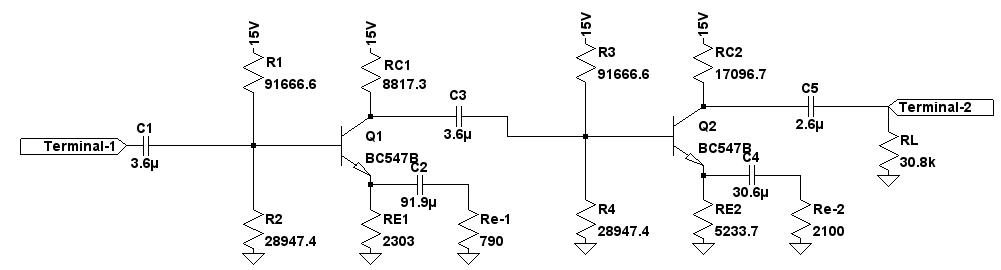
\includegraphics[scale=0.42]{maalerapporter/forforstaerker/testobjekt-forforstaerker.png}
\caption{Forforstærker med angivelser af terminaler}
\label{fig:testob_forforstaerker}
\end{figure}

\subsection*{Måleopstilling}
Målingerne foretages med to forskellige opstillinger; én til impedansmåling og én til forstærkning-, frekvensgang- og forvrængningsmåling. Opstillingerne er vist på figur \ref{fig:maaleop-imp} og figur \ref{fig:maaleop-thd}\fixme{kilde: Ole Kiel Jensen, mm5 maaleteknik}.

\begin{figure}[h]
\centering
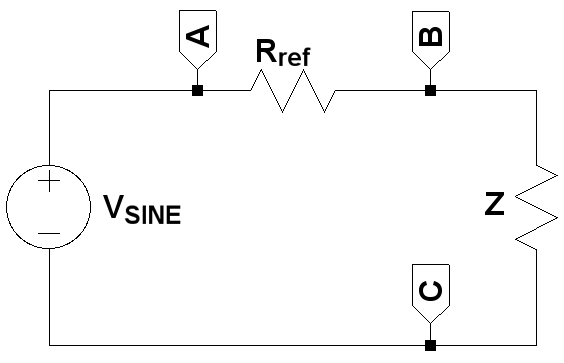
\includegraphics[scale=0.25]{maalerapporter/forforstaerker/impedansopstilling-forforstaerker.png}
\caption{Måleopstilling for impedansmåling}
\label{fig:maaleop-imp}
\end{figure}

\begin{figure}[h]
\centering
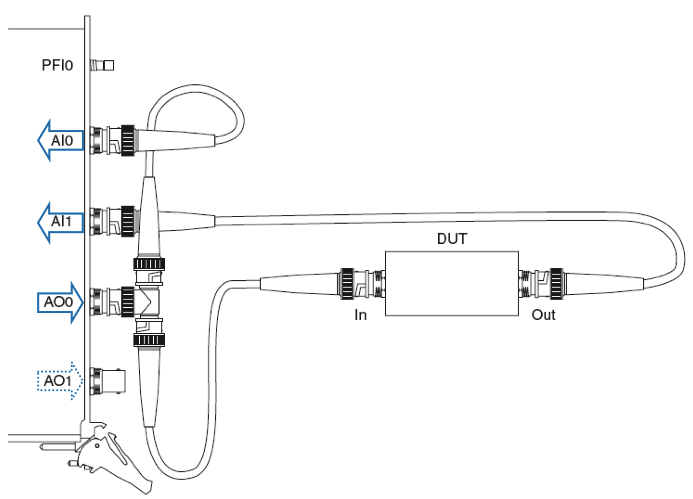
\includegraphics[scale=0.3]{maalerapporter/forforstaerker/maaleopstilling-thd-forforstaerker.png}
\caption{Måleopstilling for forstærkning-, frekvensgang- og forvrængningsmåling}
\label{fig:maaleop-thd}
\end{figure}

\subsection*{Anvendt udstyr}

\begin{table}[h]
\centering
\begin{tabular}{l|c|l}
\hline\hline
Instrument & AAU-nr. & Fabrikant, type m.v. \\
\hline\hline
Oscilloskop & 33866 & Agilent 54621A \\[4pt]
Oscillator & 07995 & B\&O RC-oscillator TG7 \\[4pt]
Spændingsforsyning & 39897 & HAMEG HM7042 \\[4pt]
Multimeter & 33048 & Fluke and Philips FLUKE 37 \\[4pt]
Audioanalysator & 76986 & National Instruments NI-PCI-4461 \\
\hline\hline
\end{tabular}
\label{tab:maaleudstyr_forforstaerker}
\end{table}

\subsection*{Måleprocedure}
Proceduren for impedansmålingen er:

\begin{enumerate}
\item Generatoren, kaldet $V_\mathrm{SINE}$ på figur \ref{fig:maaleop-imp}, indstilles til en effektivspænding på 21,1 mV (indstilles med oscilloskop) ved 1 kHz og tilsluttes
\item Reference modstanden, kaldet $R_\mathrm{ref}$ på figur \ref{fig:maaleop-imp}, vælges til 10 k\ohm~ og tilsluttes
\item Testobjektets forsyning og stel forbindes
\item Spændingsfaldet fra terminal A til terminal B, som på figur \ref{fig:maaleop-imp}, måles
\item Spændingsfaldet fra terminal B til stel, som på figur \ref{fig:maaleop-imp}, måles
\end{enumerate}

Proceduren for forstærkning-, frekvensgang- og forvrængningsmålingen er:

\begin{enumerate}
\item Spændingsforsyningen indstilles til 15 V (indstilles med multimeteret) og tilsluttes
\item Testobjektet tilsluttes som på figur \ref{fig:maaleop-thd}
\item Programmet $"$Swept Sine - Linear Response and Harmonic Distortion (DAQmx)$"$ startes
\item $"$Start frequency$"$ under Source settings sættes til 10 Hz
\item $"$Stop frequency$"$ under Source settings sættes til 25 kHz
\item $"$Amplitude$"$ under Source settings sættes til 31,6 mV
\item $"$THD units$"$ sættes til \%
\item $"$AI Range$"$ for Stimulus channel sættes til $\pm$ 0,316 V
\item $"$AI Range$"$ for Respons channel sættes til $\pm$ 3,16 V
\item $"$Sampling frequency$"$ sættes til 204,8 kHz
\end{enumerate}

Samme procedure gennemføres, hvor amplituden i punkt 6 i stedet sættes til 3,16 mV. Dermed opnåes resultater for både maksimums- og minimumsinput. 

\subsection*{Resultater}

Impedansmålingen gav effektivspændingerne vist i tabel \ref{tab:resultatimpedans_forforstaerker}. Disse spændinger bruges til at regne testobjektets indgangsimpedans, med formel (\ref{equ:zresultat-forforstaerker})\fixme{kilde: Ole Kiel Jensen, mm4 Maaleteknik}.

\begin{equation}
\label{equ:zresultat-forforstaerker}
\vert Z_\mathrm{DUT} \vert = \frac{\vert V_{Z_\mathrm{DUT}} \vert}{\vert V_{R_\mathrm{ref}} \vert} \cdot R_\mathrm{ref}
\end{equation} 

\begin{table}[h]
\centering
\begin{tabular}{l|c|c|l}
\hline\hline
 & Målt værdi & Beregnet værdi & Enhed \\
\hline\hline
$V_{R_\mathrm{ref}}$ & 6,6 & & mV effektiv\\[4pt]
$V_{Z_\mathrm{DUT}}$ & 14,6 & & mV effektiv\\[4pt]
$\vert Z_\mathrm{DUT} \vert$ & & 22,1 & k\ohm \\
\hline\hline
\end{tabular}
\caption{Resultater af impedansmåling}
\label{tab:resultatimpedans_forforstaerker}
\end{table}

Forstærkning-, frekvensgang- og forvrængningsmålingen gave resultaterne vist på figur \ref{fig:thdresultat-forforstaerker} og figur \ref{fig:fresultat-forforstaerker}.

\begin{figure}[h]
\centering
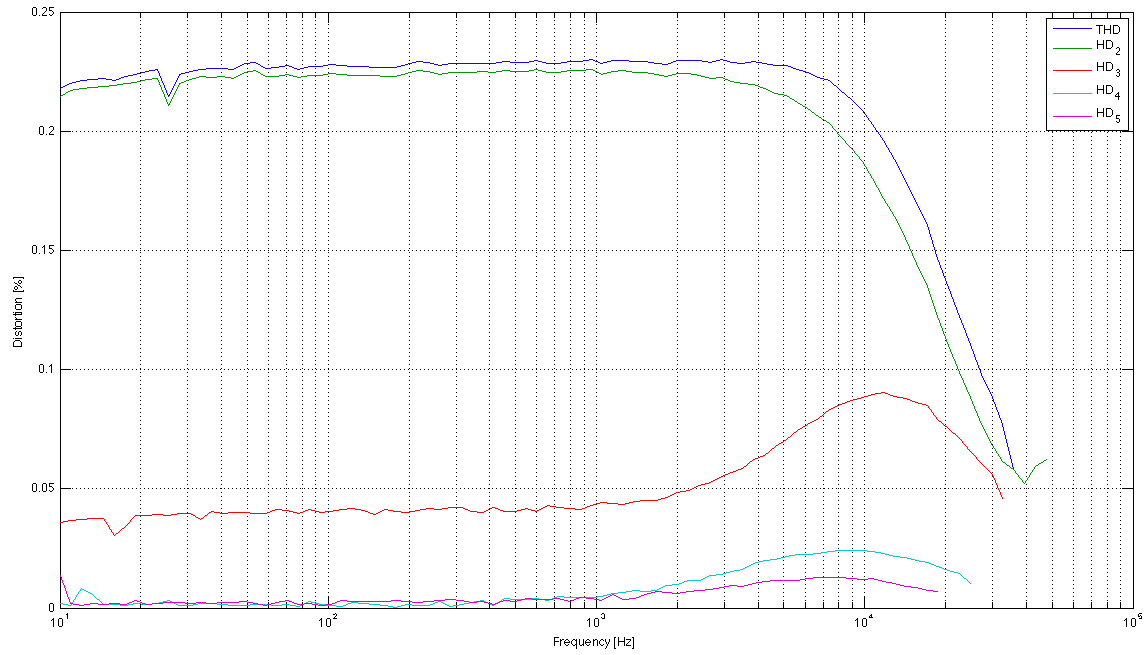
\includegraphics[width=\textwidth]{maalerapporter/forforstaerker/thd-forforstaerker.png}
\caption{Forvrængningsresultat}
\label{fig:thdresultat-forforstaerker}
\end{figure}

\begin{figure}[h]
\centering
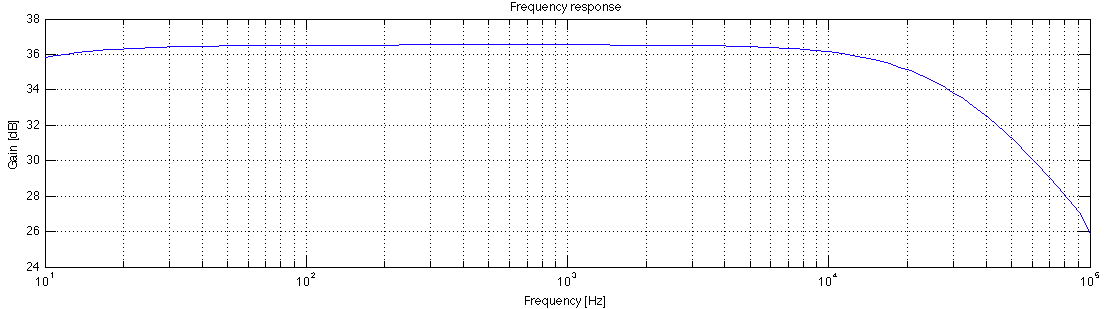
\includegraphics[width=\textwidth]{maalerapporter/forforstaerker/frekvensrespons-forforstaerker.png}
\caption{Frekvensgangs- og forstærkningsresultater}
\label{fig:fresultat-forforstaerker}
\end{figure}

Datafilerne for målingerne findes i bilag \fixme{bilag: 3.16mvInputTHDogFrekvensRespons} og \fixme{bilag: 31.6mvInputTHDogFrekvensRespons}.

\subsection*{Måleusikkerheder}
I forbindelse med målingerne er der naturligt en række usikkerheder som kan spille ind på resultaterne. Disse usikkerheder vil ikke her blive vurderet på. 

\begin{itemize}
\item Aflæsningsunøjagtigheder
\item Udstyrstolerancer
\item Måleinstrumenter belaster måleobjektet
\end{itemize}